\newpage
\section{Results}
\label{results}
The asymptotic approximation~\cite{AsymptCLs} of the LHC
$\mathrm{CL_s}$ criterion~\cite{CLs1,CLs3} is used to set upper limits on
the cross section for resonance production. The dominant sources of
systematic uncertainties are treated as nuisance parameters associated
with log-normal priors in those variables.
For a given value of the
signal cross section, the nuisance parameters are fixed to the values
that maximize the likelihood, a method referred to as
profiling. The dependence of the likelihood on parameters used to
describe the background in Eq.~(\ref{eqParam}) is treated in the same
manner, and no additional systematic uncertainty is assigned
to the parameterization of the background.


%The HP and LP event categories of H tag (V tag) are combined into a
Events from the 5 categories of Table~\ref{table:categories} 
are combined into a  
%common likelihood, with the two uncertainties in the H tag (V tag)
common likelihood, with the uncertainties of the HP and LP H tag (V tag)
efficiencies considered to be anticorrelated between HP
and LP tagging because events failing the 
HP $\tau_{42}$ ($\tau_{21}$) selection migrate to the LP category
and the fraction of events failing both HP and LP requirements is
small compared to the HP and LP events.
%of the exclusive selection on $\tau_{42}$ ($\tau_{21}$).
The branching fractions of $\Hww$ and $\Hbb$ decays
are taken as  fixed values in joint likelihood.
The remaining systematic uncertainties in the signal
are fully correlated across all channels.  The variables
describing the background uncertainties are treated as uncorrelated.
Figure~\ref{fig:HVCombined} shows 
  the observed and background-only expected upper limits
 on the production cross sections for
Z' and W', including both $\Hbb$ and $\Hww$ decays,
computed at 95\% confidence level (CL), with the predicted
cross sections for the benchmark models overlaid for
comparison. 
In the HVT model scenario B, 
W' and Z' are degenerate in resonance mass, 
thus we compute the limit on their combined cross section under this hypothesis, shown in Fig.~\ref{fig:HWHZ}.
Table~\ref{table:results} shows the
exclusion ranges on resonance masses.


\begin{table}[htb]
\begin{center}
  \caption{Summary of observed lower limits on resonance masses at 95\% CL
    and their expected values, assuming a null
    hypothesis. The analysis is sensitive to resonances heavier than 1\TeVcc.\label{table:results}}
\begin{tabular}{ ccc}
\hline
Process      & Observed & Expected \\
& lower mass limit (\TeVcc) & lower mass limit (\TeVcc) \\
\hline
${\rm W' \to HW}$ & [1.0, 1.6] & 1.7  \\
${\rm Z' \to HZ}$ & [1.0, 1.1], [1.3, 1.5] & 1.3 \\ 
%${\rm V' \to VH}$     & [1.0, 1.7], [1.9, 2.0]  & 2.0 \\
${\rm V' \to VH}$     & [1.0, 1.7] & 1.9 \\
\hline 
\end{tabular}
\end{center}
\end{table}

\begin{figure}[ht!pb]
\begin{center}
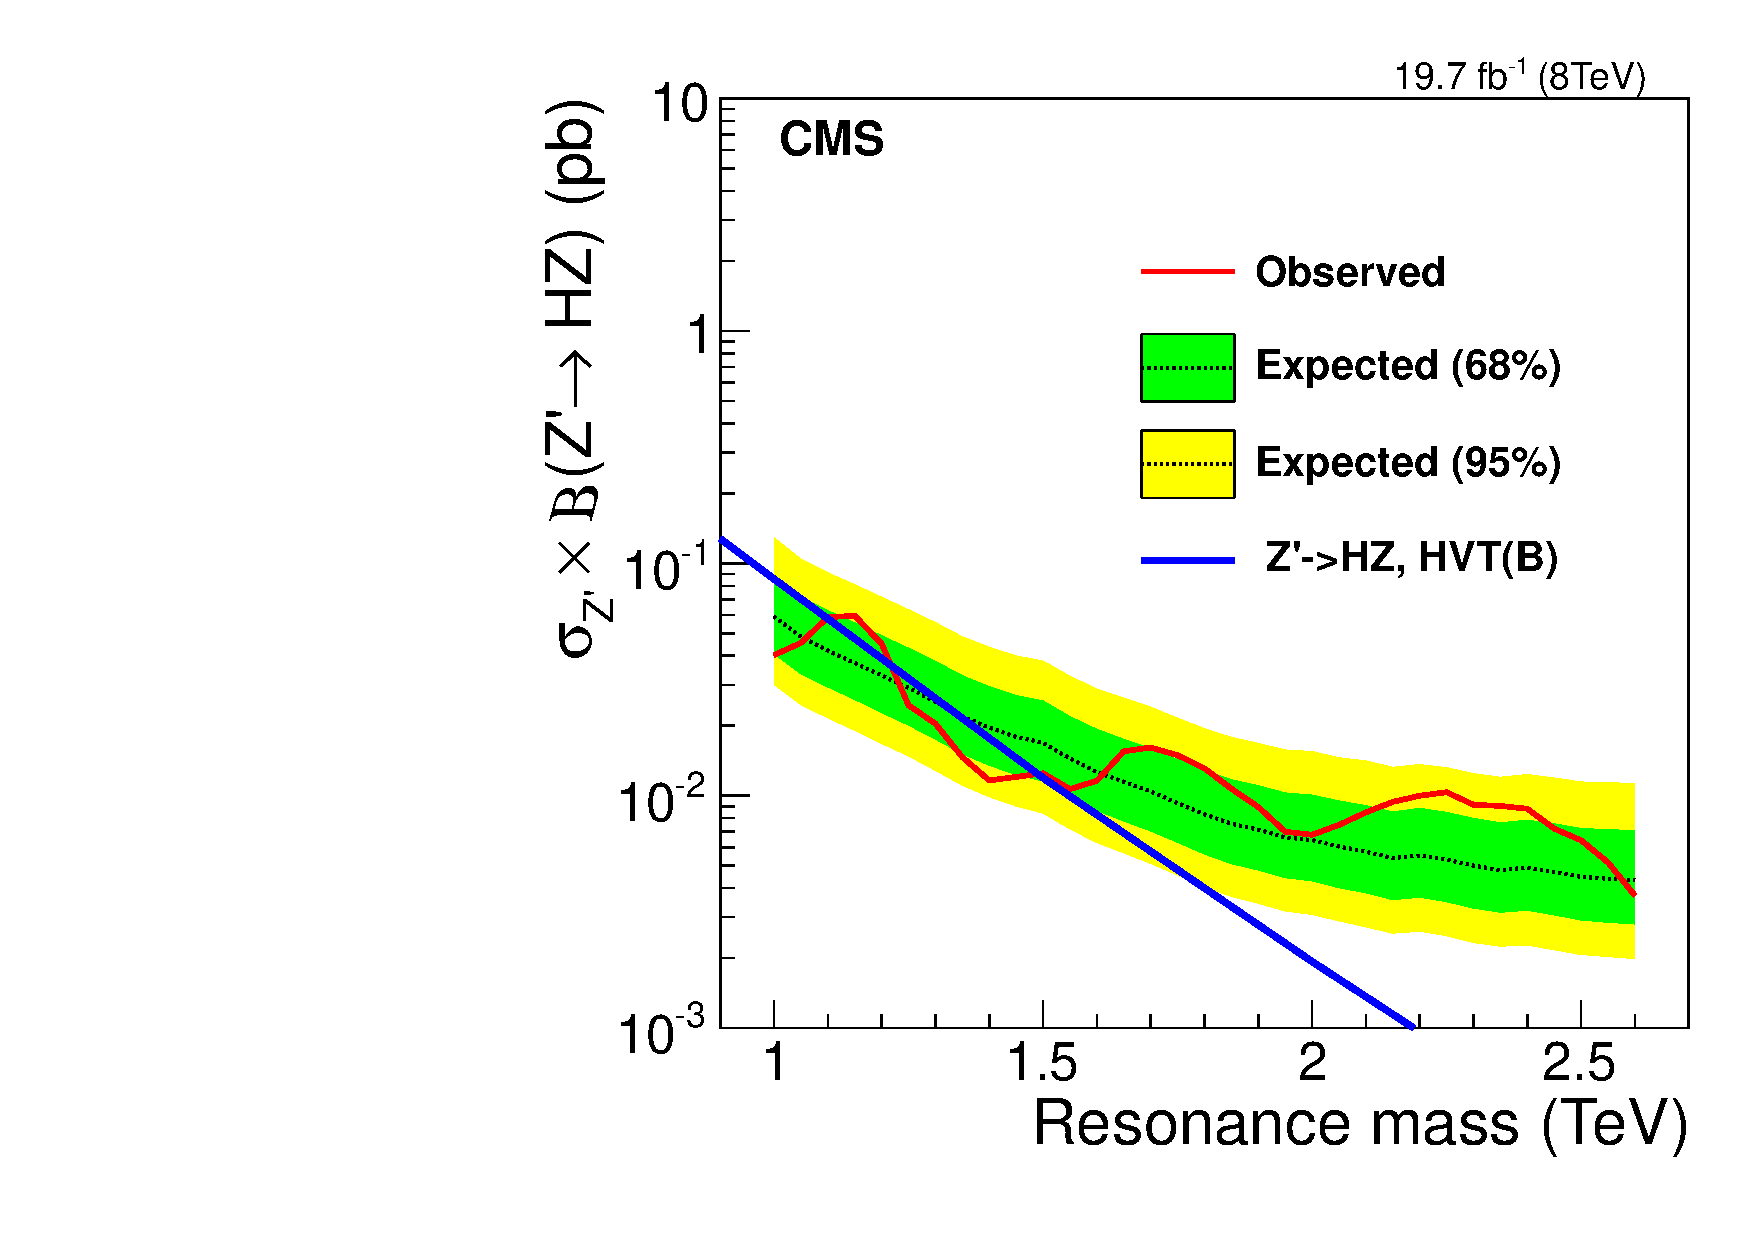
\includegraphics[width=0.49\textwidth]{EXO-14-009/figs/brazilianFlag_HZqq.pdf}
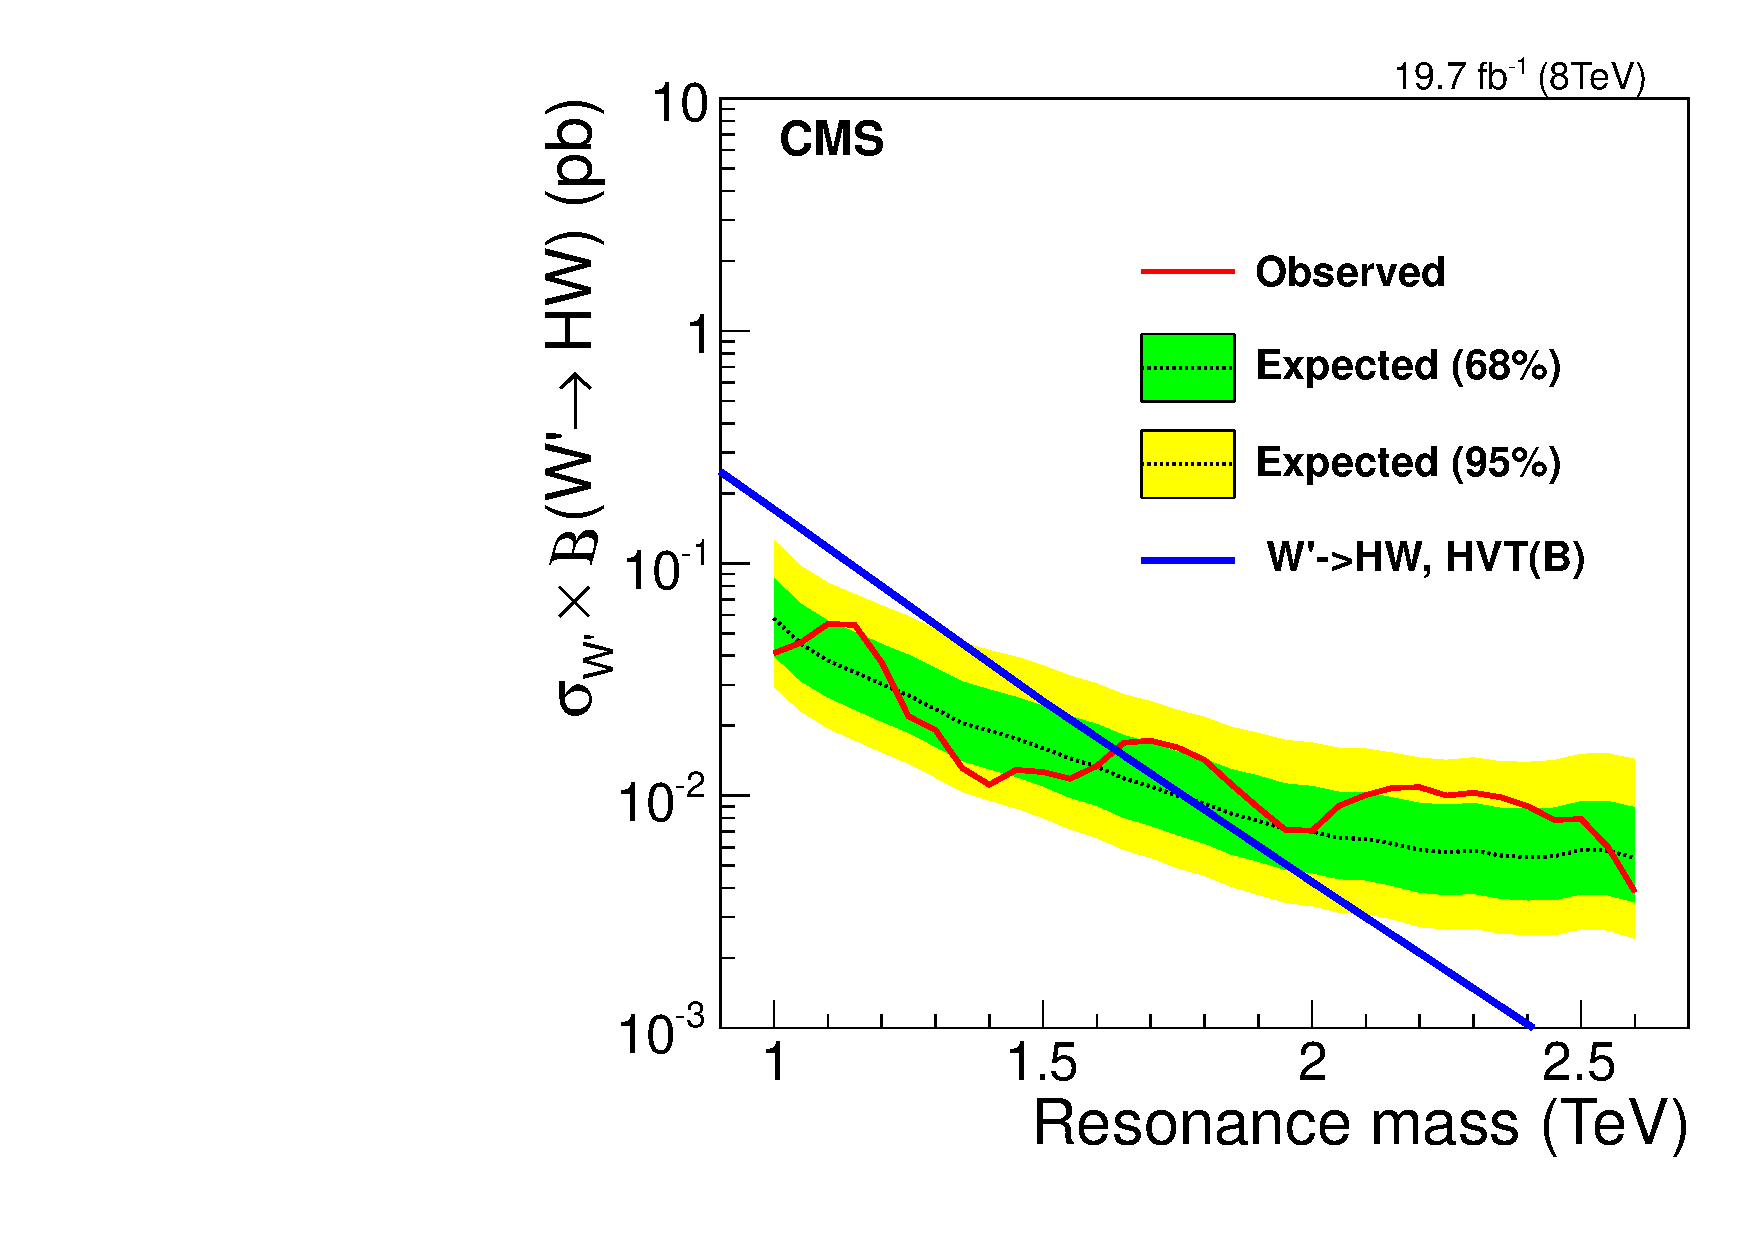
\includegraphics[width=0.49\textwidth]{EXO-14-009/figs/brazilianFlag_HWqq.pdf}
\end{center}
\caption{Expected and observed upper limits on the production 
cross sections  
for ${\rm Z'\to HZ}$ (left) and ${\rm W' \to HW}$ (right),
including all five decay categories.
 Branching fractions of H and V decays 
have been taken into account. 
 The theoretical predictions
of the HVT model scenario B are also shown.}
\label{fig:HVCombined}
\end{figure}

\begin{figure}[ht!pb]
\begin{center}
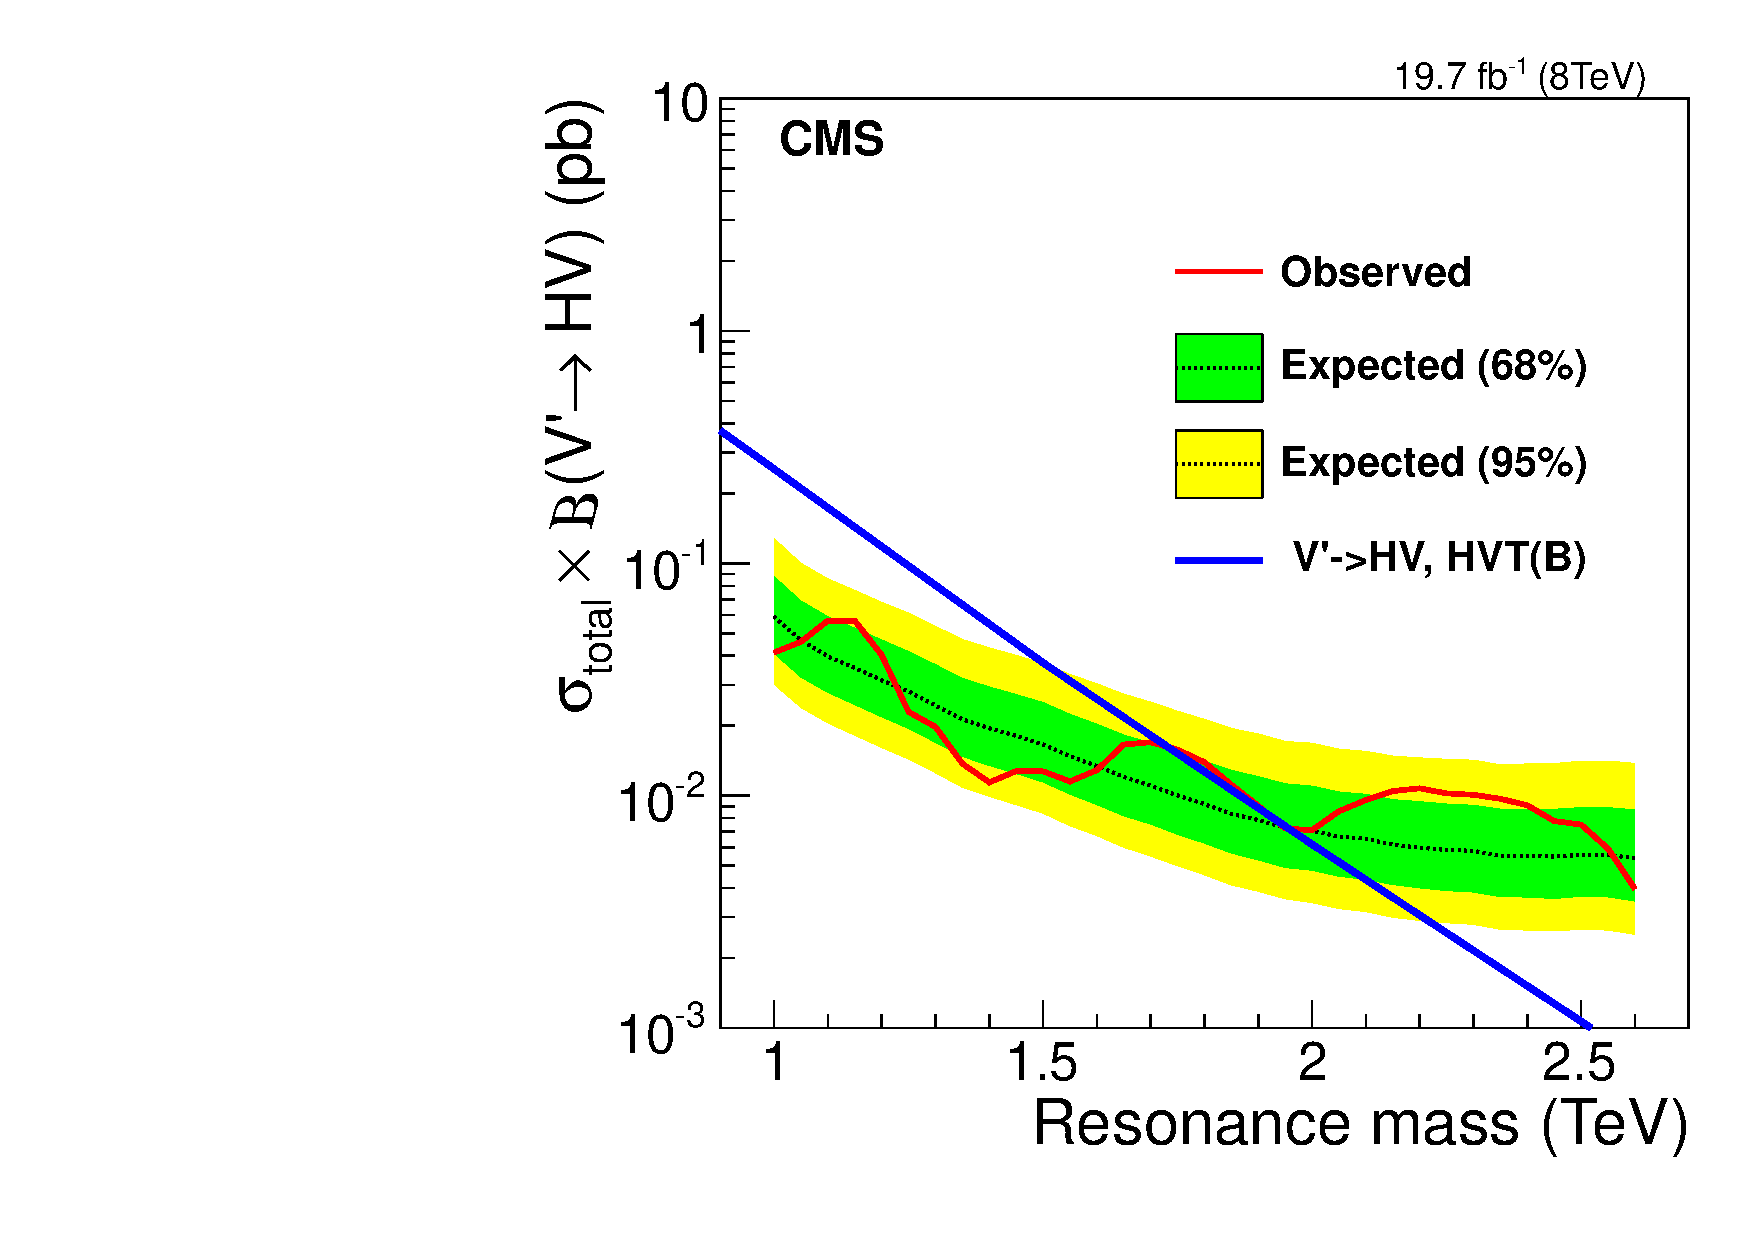
\includegraphics[width=0.60\textwidth]{EXO-14-009/figs/brazilianFlag_HV.pdf}
\end{center}
\caption{Expected and observed upper limits on the production cross section
for ${\rm V'\to VH}$,
obtained by combining W' and Z' channels together. 
 Branching fractions of H and V decays 
have been taken into account.
 The theoretical prediction
of the HVT model scenario B is also shown.
}
\label{fig:HWHZ}
\end{figure}



